\documentclass[10pt]{article}
\usepackage{graphicx}
\usepackage{wrapfig}
\usepackage{verbatim}
\usepackage{listings}


\begin{document}
\title{Assignment 2 Solutions}
\author{Vittorio Perera, Joseph Tassarotti, Wennie Tabib}
\maketitle

These experiments were run on {\tt ghc29.ghc.andrew.cmu.edu}. We could not run {\tt lshw} on the GHC machine. Here is the output of the first
process from {\tt /proc/cpuinfo}:
\begin{verbatim}
processor   : 0
vendor_id   : GenuineIntel
cpu family  : 6
model       : 44
model name  : Intel(R) Xeon(R) CPU           W3670  @ 3.20GHz
stepping    : 2
cpu MHz     : 3200.129
cache size  : 12288 KB
physical id : 0
siblings    : 12
core id     : 0
cpu cores   : 6
\end{verbatim}



\section*{Understanding the Memory Hierarchy}

\begin{center}
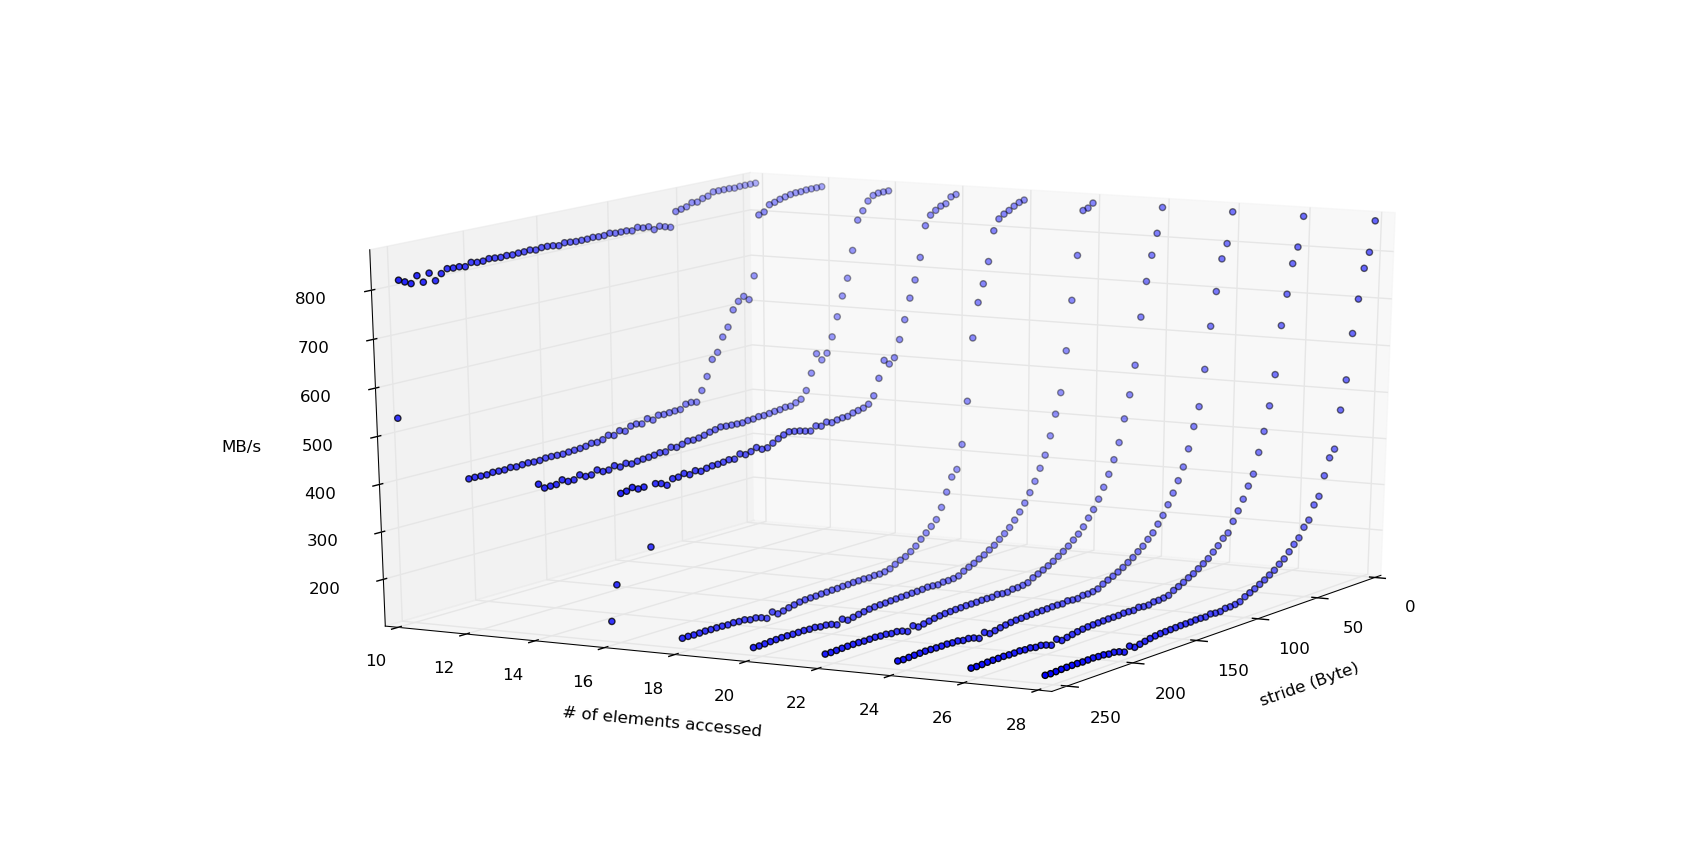
\includegraphics[scale=0.3]{images/mountain2}
\end{center}

The above image shows the output of our program in simple mode. Although one
cannot precisely determine the sizes of the cache from the plot (because we
only test powers of two for the number of elements), we can conjecture from
this graph that the linesize is between 50 and 100 bytes. Since it is probably
a power of two, we conclude it is 64 bytes. Second, looking at the drop off as
the number of elements accessed grows, we believe the L1 cache is between
$2^{10}$ or $2^12$ bytes in size, while the L2 cache is closer to $2^{16}$
bytes. 

As suggested in the assignment, we do not notice a perceptible dropoff
even as $n$ exceeds the likely size of the largest cache on the chip. We believe this
is due to prefetching -- the prefetcher anticipates the next memory access and
loads it into L3, so even though we have misses that reach L3, we never reach
DRAM.

In order to better measure the cache size, we tried various alternative access
patterns that would outsmart the prefetching strategy. For example, we
considered randomly jumping to a different location in the array every so often, or
striding through multiple rows at a time. Unfortunately, we were never able to
come up with a way to confuse the prefetcher without simultaneously loading the
cache with other irrelevant things, which itself distorts the estimate of the
cache size.

\section*{How many cores?}
We determined that there are 6 cores on the ghc machine.
You will notice that there is a tick up for every multiple of 6 cores
suggesting that there are 6 cores on the machine.
We verified this by cat'ing the /proc/cpuinfo file on the machine.

\begin{center}
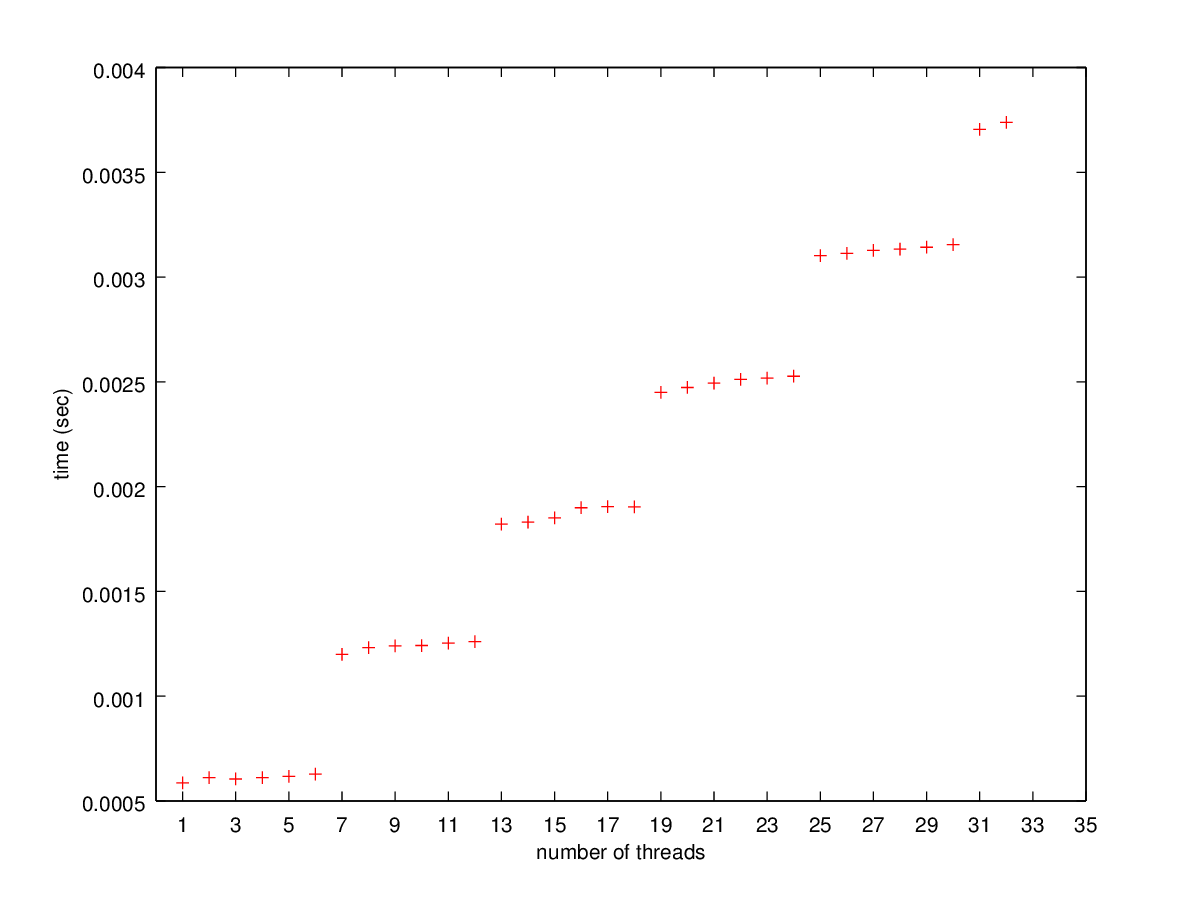
\includegraphics[scale=0.50]{images/core}
\end{center}

\section*{Determining the Shared Cache Linesize}
We determined that the line size must be 64 bytes because the program speeds up
when the distance between access locations is larger than 64 bytes.
The table can be found in output\_linesize\_ghc.txt.  For your convenience
we've also plotted the table in the graph below.

\begin{center}
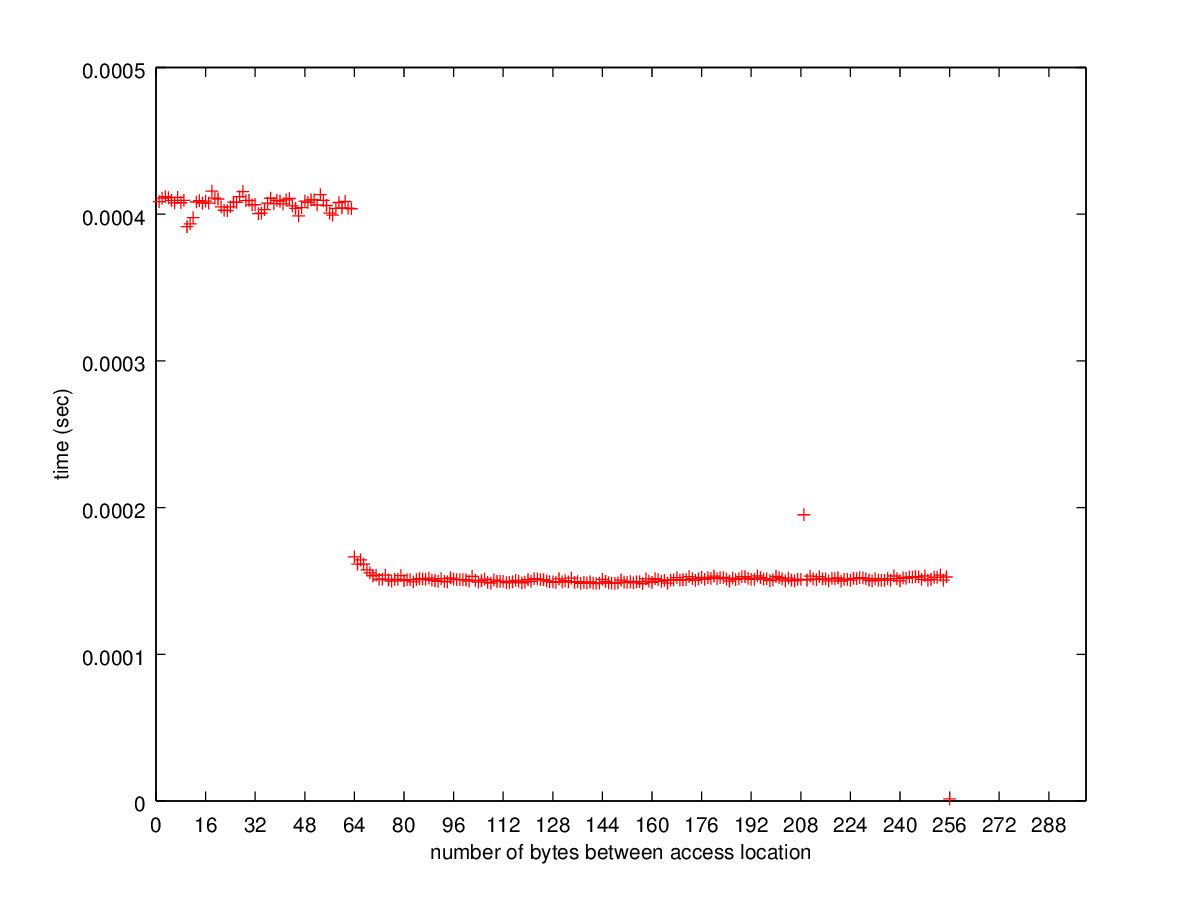
\includegraphics[scale=0.50]{images/linesize}
\end{center}

\section*{SMT or Core?}
Method to distinguish between SMT threads and number of cores:
We create a micro-benchmark in which there are memory accesses that frequently
result in misses in addition to a number of computations that need to be done
which do not depend on the memory access.

The idea here is that when multiple hyperthreads are running on the same core if
then the bubbles between their memory accesses can be filled with the
operations that do not depend on the memory accesses.

Thus when we run a second thread on the second core we will see negligible
slowdown whereas if we run out of the number of physical cores and there is no
more hyperthreading, things would slow down dramatically.

We determined that there must be there must be two SMT threads per core because
there is a noticeable dropoff at 12 and we already have evidence that there are
6 physical cores.

\begin{center}
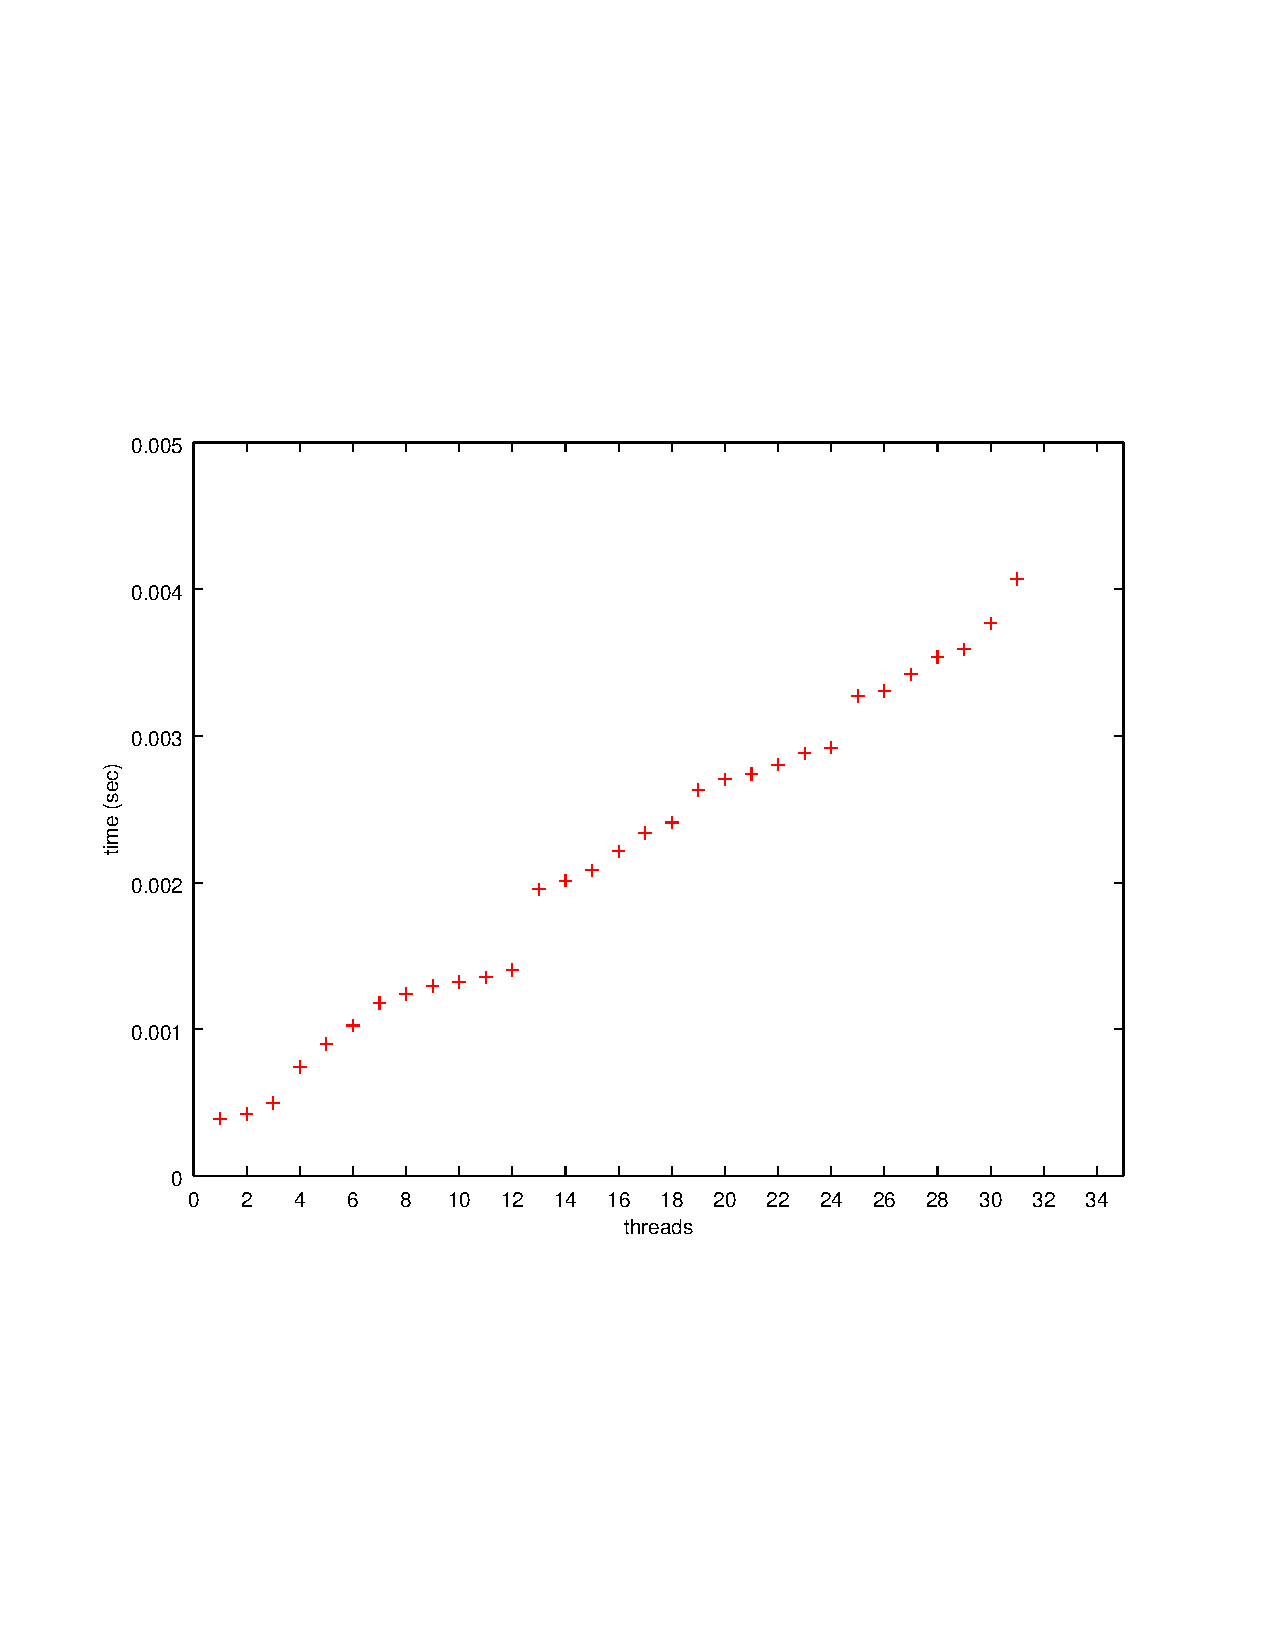
\includegraphics[scale=0.50]{images/smt}
\end{center}

\section*{A Better Lock}
Our code uses an atomic x86 instruction rather than blocking on a highly
contended lock using pthread\_lock.
Since the critical section is so small the overhead of acquiring a lock is not
worth it.
\begin{center}
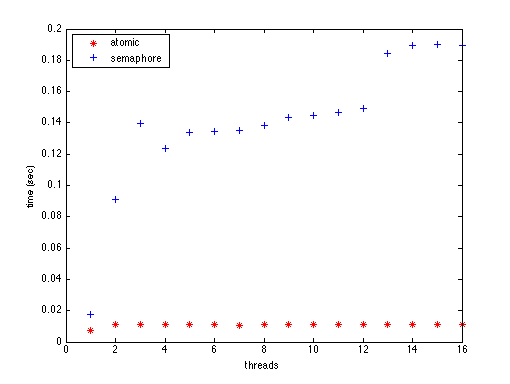
\includegraphics[scale=0.50]{images/lock}
\end{center}


\section*{Optimized Parallel Matrix Multiply}
We picked $t$ = 12 and $b$ = 16 integers on the basis of our earlier
experiments about the size of the line and the number of cores and smt threads.

The results are plotted hereafter.  
To double-check we tried changing both the number of threads and block size and
the performance got worse. In particular, we ran an experiment in which we used
6 threads instead of 12 (that is, 1 per core, without using hyperthreading).
The performance is marginally worse, for smaller matrices. We conjecture that
for larger matrices, the limited size of the cache dominates.

\begin{center}
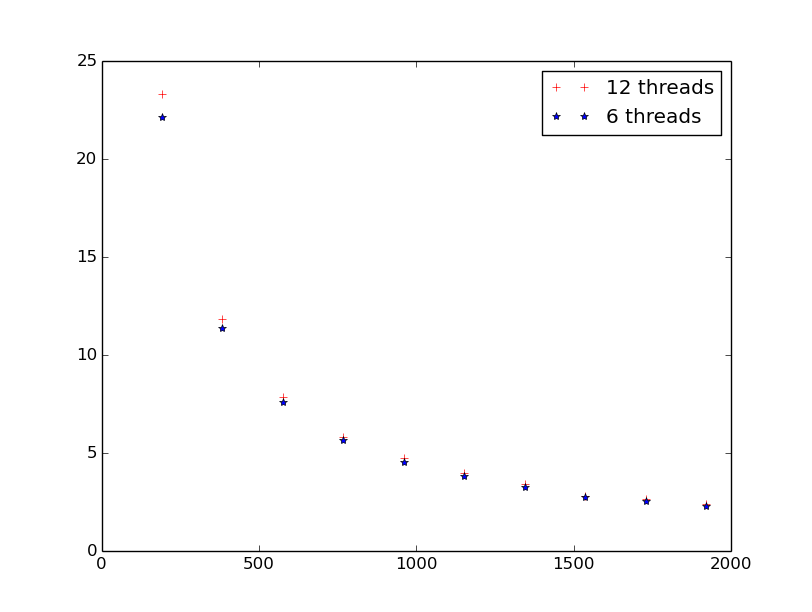
\includegraphics[scale=0.50]{images/matrix}
\end{center}





\end{document}
